
\graphicspath{ {\curdir/Graphics/}  }

Basic electrostatics requires that in free space the electric potential $\phi$ obey
\begin{equation}
	\nabla^2 \phi = 0
\end{equation}
and therefore it is impossible to have $\partial_x^2 \phi > 0$, $\partial_y^2 \phi > 0$, and $\partial_z^2 \phi > 0$ at the same point in space, which is the condition for having a stable trap in three dimensions for a positively charged particle.  The best possibility with electrostatics is to form a trap in two dimensions, but the third axis will always be an unstable equilibrium point.

Therefore to stably confine a charged particle, we have to use either static magnetic fields or time-varying electric fields.  Both of these possibilities are used in modern labs, but working with magnetostatics in Penning traps requires that the ions precess about the magnetic field axis which makes performing quantum operations on them more difficult.  All control lasers and readout must be continuously corrected for the rotation \cite{Sawyer:12,Britton:12}.  These traps are often used for precision measurements in fundamental physics \cite{Blaum:10}.  Most quantum information efforts with trapped ions use linear rf traps, which use radio frequency and dc electric fields to generate stable trapping \cite{Paul:90}.  Linear rf traps allow stationary confinement of any charged particle.

In order to more rapidly evaluate different ion trap designs, we have been working on two separate traps in different vacuum chambers.  Power from all of the necessary ionization and cooling lasers is split between the two traps.  Both chambers were originally designed to hold microfabricated surface traps, but one has been converted to hold a standard macroscopic linear rf trap in order to more easily test new quantum operations.

\section{Linear RF Traps}
\label{sec:paul}

\begin{figure}
	\centering
	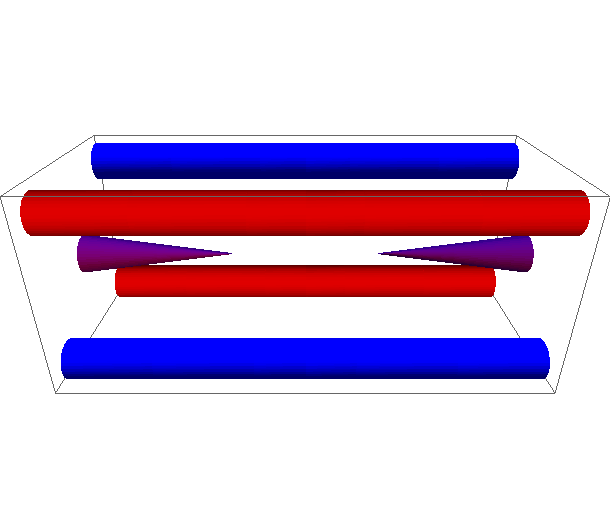
\includegraphics[width=0.8\linewidth]{PaulTrap}
	\caption[Schematic drawing of a linear rf trap]{Schematic drawing of a linear rf trap.  Radial confinement is provided by applying high voltage rf to the red rods while the blue rods are held at ground. Axial confinement is generated by applying high voltage dc to the purple needles.}
	\label{fig:paultrap}
\end{figure}

The easiest linear rf trap geometry to understand features four long rods arranged in a square with their long axis along z (see Figure~\ref{fig:paultrap}).  Radio frequency voltage is applied to two rods in opposite corners (red) and the other two rods are grounded (blue).  The rods provide radial confinement for the ions, and axial confinement is then provided by applying high voltage dc to two electrodes centered between the rods at opposite ends (purple).

At the center of the trap the rods form an oscillation radial quadrupole electric field that is a function of the angular frequency of the applied rf, $\Omega_\mathrm{rf}$, the amplitude of the rf voltage, $V_\mathrm{rf}$, and a geometrical constant, $\kappa_\mathrm{rf}$.  The resulting potential is
\begin{equation}
	\Psi_\mathrm{rf} = \kappa_\mathrm{rf} V_\mathrm{rf} \cos( \Omega_\mathrm{rf} t ) \left( x^2 - y^2 \right) \mathrm{.}
	\label{eq:pot_rf}
\end{equation}
The dc electrodes form a stable trap in the z (axial) direction, and an unstable equilibrium in x and y.  The electric potential caused by the dc electrodes at the center of the trap is
\begin{equation}
	\Psi_\mathrm{dc} = \kappa_\mathrm{dc} V_\mathrm{dc} \left( z^2 - \frac{1}{2} \left( x^2 + y^2 \right) \right) \mathrm{,}
	\label{eq:pot_dc}
\end{equation}
where $V_\mathrm{dc}$ is the dc voltage applied to both needles and $\kappa_\mathrm{dc}$ is a geometrical constant.  

The resulting axial trap frequency can easily be derived from Equation~\ref{eq:pot_dc} and is 
\begin{equation}
	\omega_z = \sqrt{ 2 \kappa_\mathrm{dc} V_\mathrm{dc} q / m }
	\label{eqn:axialfreq}
\end{equation}
for an ion of charge $q$ and mass $m$.  The equation of motion for one of the radial directions, $\hat{x}$, can be converted to the standard form of the Mathieu equation
\begin{equation}
	\frac{d^2 x}{d \xi^2} + (a_x + 2 q_x \cos(2 \xi)) x = 0 \mathrm{,}
\end{equation}
with the definitions
\begin{eqnarray}
	\xi &\equiv& \Omega_\mathrm{rf} t / 2 \\
	a_x &\equiv& \frac{4 q \kappa_\mathrm{dc} V_\mathrm{dc}}{m \Omega_\mathrm{rf}^2} \\
	q_x &\equiv& \frac{2 q V_\mathrm{rf}}{ \Omega_\mathrm{rf}^2 m } \mathrm{.}
\end{eqnarray}
Typically in experimental conditions we will have $a_x < q_x^2 \ll 1$, which results in a stable solution of the Mathieu equation.  The motion of the ion under these approximations can be written as
\begin{equation}
	x(t) = A_x \cos( \omega_x t + \phi_x ) \left( 1 + \frac{q_x}{2} \cos(\Omega_\mathrm{rf} t) \right) \mathrm{.}
	\label{eqn:mathieu-soln}
\end{equation}
The radial secular frequencies, $\omega_x$, correspond to the angular frequency of the harmonic oscillator potential the ion feels and are defined as 
\begin{equation}
	\omega_x \equiv \frac{\Omega_\mathrm{rf}}{2} \sqrt{ \frac{a_x + q_x^2/2}{1 - 3 q_x^2 / 8} } \mathrm{.}
	\label{eqn:radialfreq}
\end{equation}
The $A_x$ parameter is an amplitude set by the initial conditions of the ion.  There is still some residual motion of the ion at the frequency of the applied rf, $\Omega_\mathrm{rf}$, but the quantized motion of the ion is only described by $\omega_x$.  All of the above arguments carry through for both radial directions although I've only been discussing $\hat{x}$.  However, it is undesirable to have the radial frequencies be extremely close together because the resulting low frequency beat note makes the ions sensitive to low frequency electric field noise.  Therefore, $\omega_x$ and $\omega_y$ are usually separated either by slightly perturbing the radial symmetry of the geometry or by applying a radial symmetry-breaking dc field.

In Figure~\ref{fig:mathieu}, a solution to the Mathieu equation given a starting location near the trap center is shown.  Fast motion at the applied rf frequency, $\Omega_\mathrm{rf}$, is visible as well as the slower confining oscillation at the secular frequency, $\omega_x$.  These fast oscillations are known as trap micromotion and should be minimized as much as possible.  They lead to Doppler frequency sidebands on all lasers applied to the ion and increase ion heating when ions are moved by changing dc electrode voltages.  Additional micromotion is also induced when the ions are pushed off the quadrupole null by stray electric fields.  We will analyze micromotion further in Section~\ref{sec:secfreqs} when we work towards characterizing the secular frequencies and stray fields of a surface trap.

\begin{figure}
	\centering
	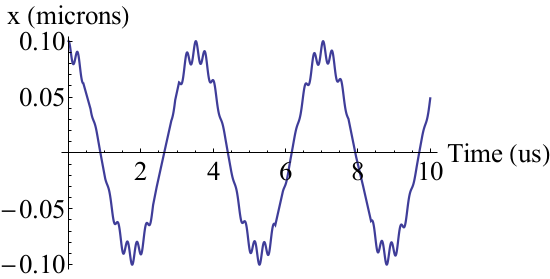
\includegraphics[width=0.8\linewidth]{PaulTrap-ion_motion}
	\caption[Sample trapped ion motion from the Mathieu equation]{Sample trajectory for an ion trapped in a linear rf trap.  The Mathieu equation is numerically integrated from a starting location near the trap center. Slow oscillation at the secular frequency and fast, driven micromotion are visible.}
	\label{fig:mathieu}
\end{figure}

When with standard macroscopic linear rf traps we have used a design exactly as pictured in Figure~\ref{fig:paultrap}.  The trap is formed by four 0.017~in (430~micron) diameter tungsten rods separated by approximately 800~microns.  The rods are held in place at either end of the trap by an alumina spacer.  In order to provide axial confinement two tungsten needles were created by electrochemically etching a fine point onto tungsten rods.  These needles are also inserted into the alumina spacers and everything is secured with a UHV-compatible cement (Sauereisen Ceramic Cement No. 8).

The rods and needles are connected to an 8-pin vacuum feedthrough.  High voltage rf to generate the trapping potential is created using a helical can resonator \cite{Siverns:12}.  Two long pieces of 3~mm diameter copper tubing are wound into a double helix of $\approx$ 4~cm diameter and 15 turns and held in the center of a 7.5~cm diameter copper can.  One end of each copper helix is connected to an rf ground and the other is connected to the vacuum feedthrough.  Rf is coupled into the resonator using a small induction coil placed inside the double helix. The shape and length of this coil can be manipulated to match the load to the standard 50~$\Omega$ output impedance of a rf amplifier.

The ground electrodes of the trap and the ends of the helix coils after the rf grounds are connected to precision dc voltage sources.  By adjusting the dc voltage of these four rods we can control the radial dc field in the trap.  These degrees of freedom allow us to cancel out any radial stray field that may be present in the trap as well as break the radial symmetry of the trap to separate the radial secular frequencies.

Although the effects of the rf are easiest to see in this type of linear rf trap geometry, many different rf and dc electrode geometries are possible.  The only requirements for this kind of trapping to work are an oscillating quadrupole electric field overlapped with dc confinement in the other directions of the correct magnitudes to correspond to a stable solution of the Mathieu equation.  A particularly simple electrode geometry is applying rf to a metal ring with dc electrodes above and below it.  Another geometry used in our group applies rf to a large parabolic mirror with a grounded metal needle inside of it \cite{Shu:11}.  The position of the ion can be manipulated by moving the needle, and by positioning it at the focus of the parabolic mirror very large fractions of the light emitted by the ion can be collected.

\section{Surface Traps}
\label{sec:surface}

A favorable geometry for working towards scalable quantum computing is called a surface electrode trap.  In this geometry, all of the electrodes are placed in a single plane.  Surface electrode traps have several advantages over standard three dimensional linear rf traps, including repeatable manufacturing processes and many separately controllable dc electrodes.  These electrodes allow the creation of separate trapping regions as well as shuttling between the regions and splitting and merging ions into them.  Many groups have been developing the techniques to design and manufacture these traps \cite{Allcock:12, Daniilidis:11, Wright:13}.

\begin{figure}
	\centering
	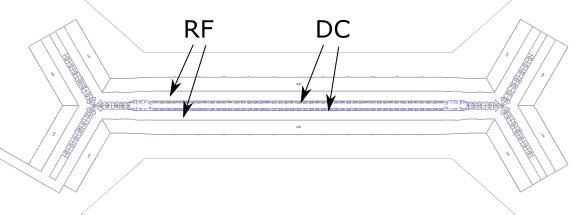
\includegraphics[width=\textwidth]{HOA}
	\caption[Electrode structure of Sandia National Lab's ``High Optical Access'' surface trap]{Electrode structure of the ``High Optical Access'' (HOA) surface trap manufactured by Sandia National Labs.  Rf voltage is applied to the long electrodes shown in red to provide radial confinement along all 5 arms of the trap.  Axial confinement is provided by applying dc voltages to the segmented electrodes between the rf electrodes.}
	\label{fig:sandia-hoa}
\end{figure}

Georgia Tech Research Institute and Sandia National Labs have provided us with microfabricated surface traps for evaluation.  The MUSIQC collaboration has been exploring a number of additional features that can be engineered into surface traps including regions of high optical access to allow tightly focused lasers, regions with optical cavities to increase ion fluorescence collection, and junctions between linear trapping regions that allow chains with different ion species composition and ordering to be organized.  Figure~\ref{fig:sandia-hoa} shows a schematic diagram of the electrodes on the trap we are currently using, the ``High Optical Access'' (HOA) trap designed and built by Sandia National Labs.  It features two junctions that allow ions to be reordered and a region in the middle where the width of the trap surface has been minimized to allow tightly focused lasers to be applied to ions from the side without clipping the trap surface.  In order to be able to evaluate different trap designs quickly we have designed and implemented a vacuum chamber that allows for quick trap replacement \cite{Graham:14}.

The surface electrode traps we receive are wirebonded onto a CPGA-100 carrier.  This carrier slots into a UHV-compatible Zero Insertion Force (ZIF) socket in the center of our vacuum chamber (see Figure~\ref{fig:chipchamber}).  The ZIF socket connects to a custom PCB that can, if necessary, host additional filtering for the dc voltages that will be applied to the trap.  The PCB also routes the connections from the socket to four 25~pin D-Sub connectors that are connected through a vacuum feedthrough to our control electronics.  The neutral atom ovens mount below the PCB.  The bottom flange of the vacuum chamber can be removed to replace the oven, and the top flange can be removed to replace the trap.  This system has been cycled from atmospheric pressure to pressures below 5~$\times$~10$^{-11}$~torr more than ten times, often in a week or less.

In order to minimize the deposition of metallic barium and ytterbium from the ovens on the back of the surface trap we have developed several techniques to shutter the ovens in the vacuum chamber.  The shutter can be activated before running the oven at very high temperatures to remove material deposited during the bake out of the UHV chamber.  These high temperature runs are necessary before the oven will produce a usable flux of the element to be ionized.  We have seen evidence that during these runs barium ovens can eject pieces large enough to completely block the loading holes on surface electrode traps.  The shutter shown in Figure~\ref{fig:chipchamber} is made of a small metal plane attached to a bimetallic strip that curls when its temperature is increased.  By running several amperes of current through the bimetallic strip the plane can be actuated to block flux from the oven below the surface trap.

\begin{figure}
	\centering
	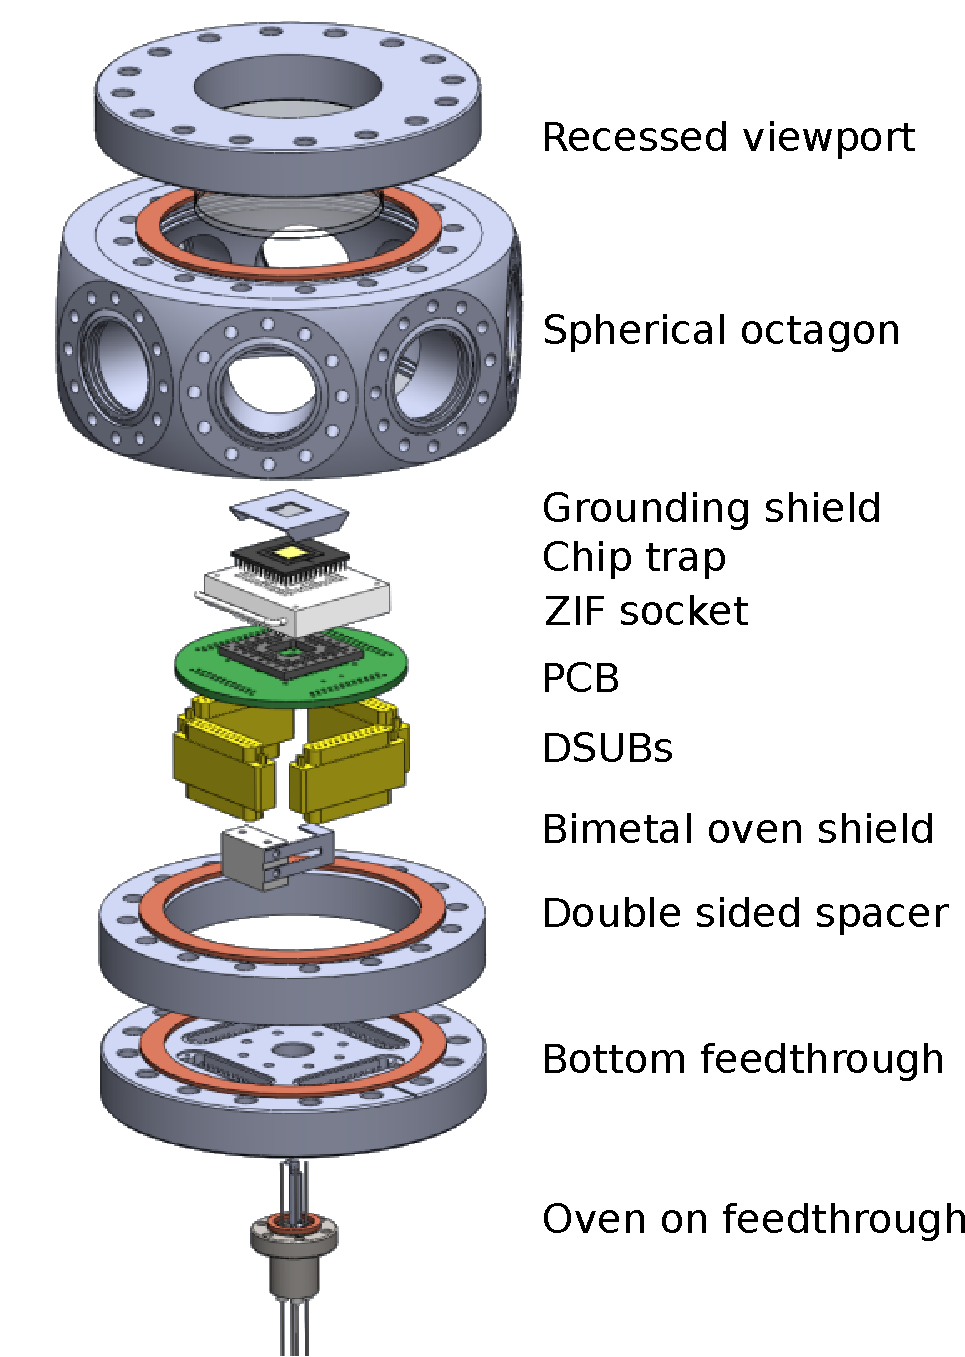
\includegraphics[width=0.7\textwidth]{chiptrap-chamber}
	\caption[Diagram of surface trap vacuum chamber]{Diagram of vacuum chamber designed for working with surface traps.  The surface trap mounts in a ZIF socket and its electrical connections are routed through 4 25-pin D-Sub connectors.  Barium and ytterbium ovens are located below the trap and can be blocked with a bimetal shutter.}
	\label{fig:chipchamber}
\end{figure}

The next step to begin working with these microfabricated traps is to calculate the correct voltage to apply to each dc electrode to generate a stable axial trap.  The electric fields at the trapping location in surface traps as a function of the applied dc voltages are often calculated using the Boundary Element Method (BEM).  All of the surfaces in the trap are subdivided into small triangles or quadrilaterals and a surface charge degree of freedom is placed at each vertex of this mesh.  In the lowest order approximation, the actual surface charge is assumed to be the linear interpolation of the surface charge at these points. These steps reduce the problem from one large integral to the sum of a large number of integrals that depend linearly on the surface charge at each vertex.  In other words, the problem of solving for the electric potential, $\phi$, is changed from
\begin{equation}
	\phi(x) = \int_{\{S\}} \frac{\sigma(x')}{4 \pi \epsilon_0 \left| x - x' \right| } dx' \mathrm{,}
\end{equation}
where $\sigma(x)$ is the surface charge density and $\{S\}$ is the set of surfaces in the trap, to the more numerically tractable
\begin{equation}
	\phi(x_i) = \sum_{S_k = x_q, x_r, x_s} \int_0^1 \int_0^v \frac{(1-u-v)\sigma(x_q) + u\sigma(x_r) + v\sigma(x_s)}{4 \pi \epsilon_0 \left| x_{S_k}(u, v) - x_i \right| } \left| \frac{\partial x}{\partial (u,v)} \right| du dv \mathrm{,}
\end{equation}
where $u$ and $v$ are a linear parametrization of the small triangular surface $S_k$, defined by the three vertices $x_q$, $x_r$ and $x_s$, such that $x_{S_k}(0, 0) = x_q$, $x_{S_k}(1, 0) = x_r$, and $x_{S_k}(0, 1) = x_s$.  The $S_k$ triangles are chosen to approximate the surfaces $\{S\}$ to the desired level of accuracy.  The desired solution is then a set of $\sigma(x_i)$ given a desired set of voltages on each surface $\phi(x_i)$ where both of these functions are only evaluated at the vertices of the mesh.

The problem of solving for these vertex surface charges can then be reduced to linear algebra by computing the integrals 
\begin{eqnarray}
	U_{ij} &=& \int_0^1 \int_0^v \frac{u}{4 \pi \epsilon_0 \left| x_{S_j}(u, v) - x_i \right| } \left| \frac{\partial x}{\partial (u,v)} \right| du dv \\
	V_{ij} &=& \int_0^1 \int_0^v \frac{v}{4 \pi \epsilon_0 \left| x_{S_j}(u, v) - x_i \right| } \left| \frac{\partial x}{\partial (u,v)} \right| du dv 
\end{eqnarray}
for every vertex $x_i$ and every triangle $S_j$.  Then, given the desired voltages on each surface, the resulting surface charge distribution can be calculated by standard linear algebra techniques.  We have developed software that performs the integration using Gaussian quadrature, and inverts the generated matrix using the open source PETSc\footnote{Portable, Extensible Toolkit for Scientific Computation - \url{http://www.mcs.anl.gov/petsc/}} package.

\begin{figure}
	\begin{tabular}{ccc}
		\centering
		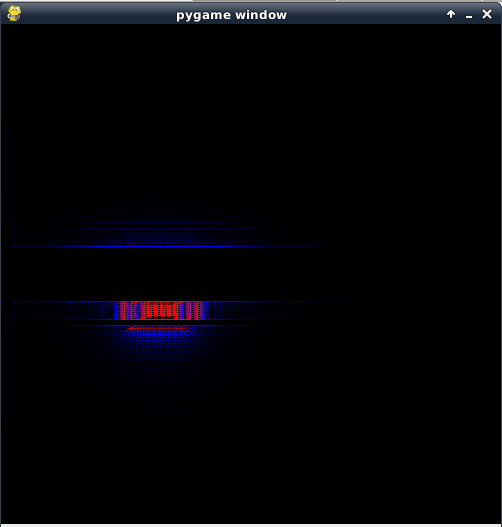
\includegraphics[width=0.3\textwidth]{dc_5} &
		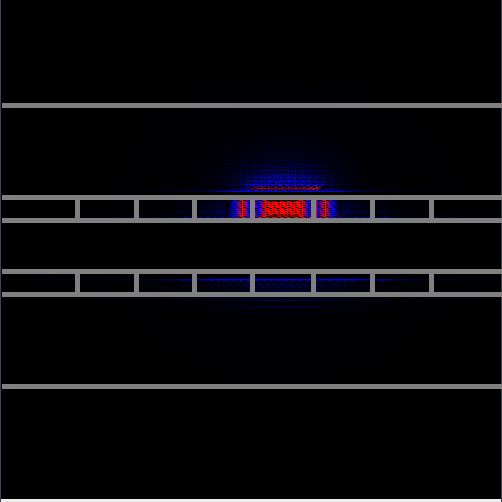
\includegraphics[width=0.3\textwidth]{dc_10} &
		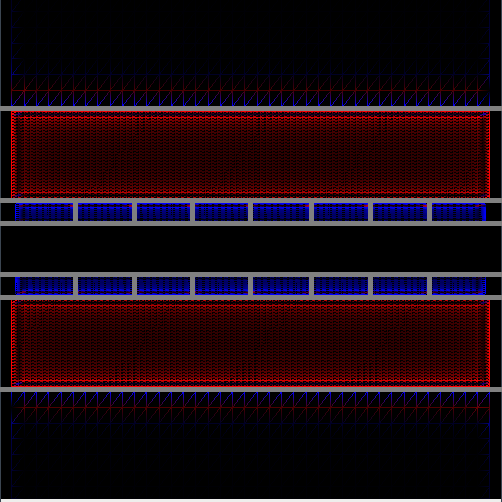
\includegraphics[width=0.3\textwidth]{rf_rails} \\

		
\includegraphics[width=0.3\textwidth]{yz_5} &
		
\includegraphics[width=0.3\textwidth]{yz_10} &
		
\includegraphics[width=0.3\textwidth]{yz_rf}
	\end{tabular}
	\caption[Electric potentials for sample electrodes in a surface trap]{Electric potential in the center of the Sandia HOA trap caused by charging individual electrodes.  The upper panels show the induced surface charges on the trap electrodes and the lower panels show the electric potential in the vertical and axial directions found using the BEM method.  The left and center panels are for two different dc electrodes, while the right panel shows the pseudopotential resulting from the rf electrode.}
	\label{fig:BEMpots}
\end{figure}

Usually in order to be able to quickly analyze voltage solutions the electric field of each electrode is solved individually (see Figure~\ref{fig:BEMpots}).  Every electrode is set to 0~V except for one which is assigned some nominal value, for example 1~V.  The total electric field for a set of voltages can then be found using superposition by scaling and adding these results for each electrode.  The radial trapping potential is analyzed by performing the same analysis for the rf electrodes and then calculating the electric field from this analysis.  The radial behavior of the ion can be described by an rf pseudopotential approximation
\begin{equation}
	\phi_{\mathrm{pseudo}} = \frac{q}{4 m \Omega_\mathrm{rf}^2}\left| \nabla \vec{E} \right| ^2
\end{equation}
where $\vec{E}$ is the electric field vector, $q$ is the charge of the ion, $m$ is the ion mass, and $\Omega_\mathrm{rf}$ is the frequency of the applied rf voltage.  The secular motion of the ion is described by this potential under the same approximations that we made before, but micromotion is not taken into account.  The minimum of the potential and its harmonic coefficients are found by repeatedly fitting the potential at a trial point to a second order polynomial in three dimensions and moving the trial point along the linear gradient \cite{Blakestad:11}.  When the linear terms are minimized, the bottom of the potential has been found and the harmonic terms can be found by diagonalizing the second order polynomial.

Multidimensional functional minimization is then used to find voltage solutions with desired trap strengths and locations.  Ions can be shuttled axially by solving for voltages that generate a trap every few microns along the region of interest.  Applying these solutions in order at some sufficiently high fixed speed will shuttle the ion at roughly constant velocity.  Stray fields in surface traps can be compensated by finding combinations of voltages that produce electric fields in each direction at the trapping location.  Scaling and combining these electric field generating voltages allows us to cancel any stray field.

Once a trapping potential has been calculated, it must be applied to the dc electrodes.  The current generation of traps have up to 96 dc electrodes that must be independently controlled.  After evaluating potential solutions, including using many 8 channel National Instruments cards in a PCI chassis or a hundred separate high precision DAC chips, we decided to implement a solution using a few many-channel DAC chips.  The AD5372 is an Analog Devices chip that contains 32 independent DACs with 16-bit precision and 20~V output range.  The latter two specifications are sufficient for our needs and, with 32 channels each, three chips suffice to control any of the current generation surface electrode traps.

The disadvantage of using a many-channel chip is that it is not possible to update the voltages of all of the electrodes simultaneously.  Each chip supports a serial interface at 50~MHz and a minimum time between channel updates of 600~ns.  To perform a single step in a shuttling solution it is necessary to update 8 to 10 adjacent electrodes.  These updates must be sent sequentially to separate channels on a single DAC chip which limits the overall update rate to $\approx$ 200~kHz.  The AD5372 does include the functionality to buffer all of the channel updates in a single shuttling step into its registers and then present the voltages simultaneously to the ion trap.  The potential the ion sees is never in an intermediate state and always corresponds to one of the potentials in the solution file even though the updates are communicated serially to the DAC board.

Communication with the DAC chips is accomplished through their serial interface using a custom FPGA software solution implemented on an Altera DE2-115 FPGA development board.  This board features 512~KB of SRAM and a DM9000a ethernet controller.  In order to shuttle the ion, the lab computer loads the shuttling solution from files and transmits it via UDP to the DM9000a ethernet controller.  The FPGA board stores each solution step in SRAM and confirms its receipt to the lab computer.  Once the solution has been loaded it can be played from any desired step to any other at the maximum update rate of the DAC chips by the FPGA.  Since each step could take a different number of channel updates and it is desirable to maintain the same time period between steps in the shuttling solution file the FPGA will automatically generate delays if necessary between solution steps.

Using this system we have successfully trapped barium ions in two different surface electrode traps and have demonstrated shuttling ions.  In order to work on ions at different positions along the axis we have also developed computer controlled systems for positioning the cooling lasers and imaging systems.  We currently shift the position of the cooling lasers using a mirror with a piezoelectric control system.  A custom dc-dc amplifier transforms voltages from an ADC output from a microcontroller into a high voltage input for the piezo mirror.  The microcontroller communicates with the experimental control computer over a serial interface, and it can be program to any desired voltage or to sweep over multiple voltages spending a designated amount of time at each voltage.  This second mode is useful for working on multiple trapping regions at the same time.

In this chapter we have described all of the technology we will need to trap ions for the rest of this work.  Macroscopic linear rf traps are useful for easily evaluating new techniques because of their lower heating rates and easier optical access.  Surface traps will enable us to work with larger numbers of ions and to work efficiently with multiple ion species.  The next two pieces of setup we need are the ionization lasers and the cooling lasers that will create and cool our ions and maintain their low temperatures.  I will discuss these in the next chapter.
